\documentclass[11pt]{scrartcl}
\usepackage{polski}
\usepackage[polish]{babel}

\usepackage{graphicx, float, caption, subcaption, amsmath}
\usepackage{tabularx, multirow, hyperref, enumitem, listings}
\usepackage{xcolor}
%\usepackage{minted}

\hypersetup{
    colorlinks=true,
    linkcolor=black,
    urlcolor=black,
    citecolor=black
}

\definecolor{md-black}{rgb}{0.12, 0.12, 0.12}
\definecolor{md-teal}{rgb}{0.38, 0.79, 0.69}
\definecolor{md-mauve}{rgb}{0.76, 0.52, 0.75}
\definecolor{md-yellow}{rgb}{0.86, 0.86, 0.67}
\definecolor{md-green}{rgb}{0.13, 0.55, 0.13}
\definecolor{md-red}{rgb}{0.82, 0.10, 0.14}
\definecolor{md-purple}{rgb}{0.69, 0.33, 0.73}
\definecolor{md-orange}{rgb}{0.96, 0.42, 0.18}
\definecolor{md-gray}{rgb}{0.44, 0.46, 0.51}
\lstset{
    language=Python,
    basicstyle=\color{md-teal}\ttfamily,
    keywordstyle=\color{md-mauve},
    commentstyle=\color{md-green},
    stringstyle=\color{md-red},
    numbers=left,
    numberstyle=\small\color{md-gray}\ttfamily,
    stepnumber=1,
    numbersep=5pt,
    backgroundcolor=\color{md-black},
    showspaces=false,
    showstringspaces=false,
    showtabs=false,
    frame=none,
    tabsize=4,
    captionpos=b,
    breaklines=true,
    breakatwhitespace=false,
    escapeinside={\%*}{*)},
    numbersep=-10pt,
    morekeywords={as},
    classoffset=1,
    morekeywords={quad, trapz, simps},
    keywordstyle=\color{md-yellow},
    classoffset=0
}

\graphicspath{{images/}}

\title{Laboratorium 6 - Kwadratury}
\author{Mateusz Podmokły - II rok Informatyka WI}
\date{11 kwiecień 2024}

\begin{document}
    \maketitle
    \section{Treść zadania}
    \textbf{Zadanie 1.} Wiadomo, że
    \[
        \int_{0}^{1}\frac{4}{1+x^2}dx=\pi
    \]
    Oblicz wartość powyższej całki, korzystając ze złożonych
    kwadratur otwartej prostokątów (ang. mid-point rule),
    trapezów i Simpsona. Na przedziale całkowania rozmieść
    $2^m+1$ równoodległych węzłów. Przyjmij zakres
    wartości $m$ od 1 do 25. Dla każdej metody narysuj wykres
    wartości bezwzględnej błędu względnego w zależności od
    liczby ewaluacji funkcji podcałkowej $n$.
    \subsection*{}
    \textbf{Zadanie 2.} Oblicz wartość całki
    \[
        \int_{0}^{1}\frac{4}{1+x^2}dx
    \]
    metodą Gaussa-Legendre'a. Narysuj wykres wartości bezwzględnej
    błędu względnego w zależności od liczby ewaluacji funkcji
    podcałkowej $n$.

    \section{Specyfikacja użytego środowiska}
    Specyfikacja:

    \begin{itemize}
        \item Środowisko: Visual Studio Code,
        \item Język programowania: Python,
        \item System operacyjny: Microsoft Windows 11,
        \item Architektura systemu: x64.
    \end{itemize}

    \section{Rozwiązanie problemu}
    \subsection{Biblioteki}
    W realizacji rozwiązania wykorzystane zostały następujące
    biblioteki:
    \begin{lstlisting}
        import numpy as np
        import matplotlib.pyplot as plt
        from scipy.integrate import trapz
        from scipy.integrate import simps
    \end{lstlisting}

    \subsection{Zadanie 1.}
    Każda z metod całkowania numerycznego przybliża całkę w nieco
    inny sposób. Poniżej krótkie wyjaśnienie każdej z użytych
    metod.
    \subsubsection{Metoda prostokątów}
    Całka została obliczona według następującego wzoru:
    \[
        \int_{a}^{b}f(x)dx \approx \sum_{i=0}^{n-1}hf
        \left( a+ \left( i+\frac{1}{2} \right) \cdot h \right)
    \]
    gdzie
    \[
        h=\frac{b-a}{n}
    \]

    \subsubsection{Metoda trapezów}
    Do obliczenia całki metodą trapezów została wykorzystana funkcja
    z biblioteki \texttt{SciPy}
    \[
        \texttt{scipy.integrate.trapz}
    \]
    \subsubsection{Metoda Simpsona}
    Do obliczenia całki metodą Simpsona została wykorzystana funkcja
    z biblioteki \texttt{SciPy}
    \[
        \texttt{scipy.integrate.simps}
    \]

    \subsection{Zadanie 2.}
    \subsubsection{Metoda Gaussa-Legendre'a}
    Metoda oblicza wartość całki na przedziale $[-1,1]$
    w następujący sposób:
    \[
        \int_{-1}^{1}f(x)dx \approx \sum_{i=1}^{n}w_if(x_i)
    \]
    gdzie $w_i$ to wagi kwadratury, a $x_i$ to pierwiastki
    i-tego wielomianu Legendre'a. Można je wyznaczyć korzystając
    z funkcji \texttt{np.polynomial.legendre.leggauss}. \\
    Całka w zadaniu zdefiniowana jest na przedziale $[0,1]$, więc
    musimy zastosować podstawienie
    \[
        x=\frac{1}{2}t+\frac{1}{2}
    \]
    aby uzyskać przedział całkowania $[-1,1]$. Po obliczeniu całki
    należy przywrócić początkową szerokość przedziału dzieląc wynik
    przez 2. Wtedy wzór przyjmuje postać
    \[
        \int_{0}^{1}f(x)dx \approx \frac{1}{2}\sum_{i=1}^{n}w_i
            f \left( \frac{1}{2}t+\frac{1}{2} \right)
    \]

    \section{Przedstawienie wyników}
    \subsection{Zadanie 1.}
    \begin{figure}[H]
        \centering
        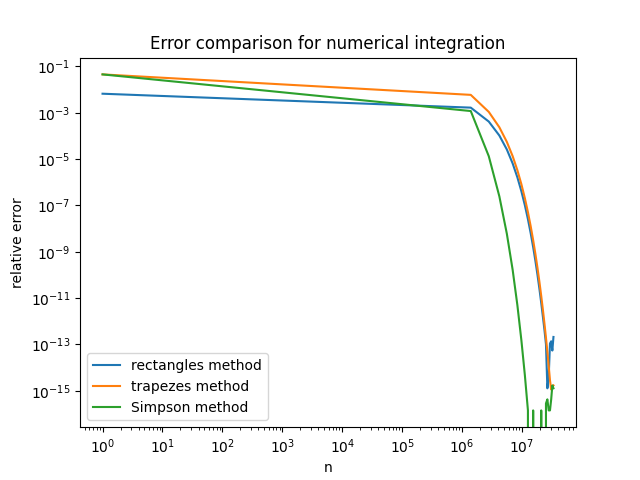
\includegraphics[width=0.8\linewidth]{integration_err.png}
        \caption{Wartości błędu względnego dla różnych metod
        całkowania.}
    \end{figure}

    Od $n \approx 10^7$, czyli $h \approx 10^{-7}$, zwiększanie
    wielkości kroku $h$ nie zmniejsza już błędu kwadratury. Pomiary
    z Laboratorium 1. wynosiły $h_{min} \approx 10^{-8}$ oraz $h_{min}
    \approx 10^{-6}$. Wartości $h_{min}$ z obydwu laboratoriów są do
    siebie zbliżone.

    \subsection{Zadanie 2.}
    \begin{figure}[H]
        \centering
        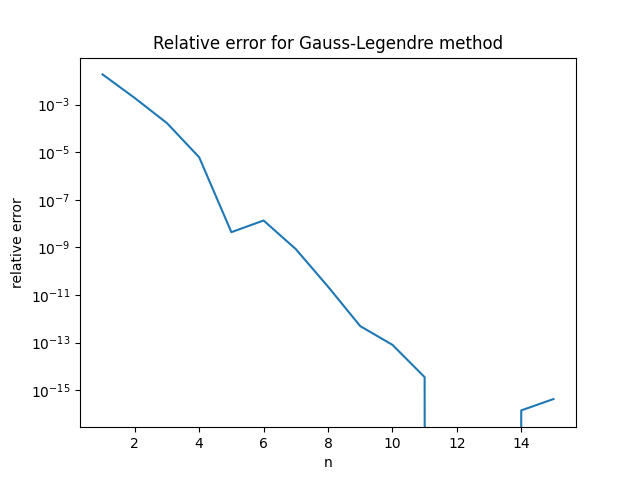
\includegraphics[width=0.8\linewidth]{gauss-legendre_err.png}
        \caption{Wartości błędu względnego dla metody
        Gaussa-Legendre'a.}
    \end{figure}

    \section{Wnioski}

    \section{Bibliografia}
    \url{https://pl.wikipedia.org/wiki/Ca%C5%82kowanie_numeryczne} \\
    \url{https://pl.wikipedia.org/wiki/Kwadratury_Gaussa} \\
    \url{https://pl.wikipedia.org/wiki/Wielomiany_Legendre%E2%80%99a} \\
    \url{https://www.fuw.edu.pl/~jnareb/zajecia/int-gauss.pdf}

\end{document}
